\section{Funktionsweise und Frequenzgang eines Integrators}
Bei diesem Versuch wird ein Integrator aufgebaut mittels des Operationsverstärker. Der Aufbau erfolgt nach der Abbildung \ref{fig:Versuch2/Schaltbild eines Integrators} in die Schaltung wird für R= 1 $k \Omega$ und C= 10 $nF$ genommen, welche vorher gemessen werden mittels eines Multimeters und die Fehler können als vernachlässigbar angesehen werden. Der Sweep-Modus wird im Funktionsgenerator ausgeschaltet sowie wird eine Frequenz von 1 $kHz$, eine Amplitude von 500 $mV$ und einen DC-Offset von 0 $V$ eingestellt. Mit dem Oszilloskop wird dann die Eingangsspannung $U_1$ und die Ausgangsspannung $U_2$ des Operationsverstärkers gemessen und werden die Bilder einer Rechteckspannung, einer Dreiecksspannung und einer Sinusspannung mit der integrierte Form, die über die Ausgangsspannung $U_2$ ausgegeben wird, gespeichert.   
\begin{figure}[H]
    \centering
    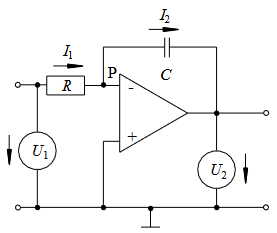
\includegraphics[width=0.4\textwidth]{Funktionsweise und Grequenzgang eines Integrators Aufbau.png}
    \caption{Schaltbild eines Integrators, entnommen aus \cite{script}}
    \label{fig:Versuch2/Schaltbild eines Integrators}
\end{figure}
In der Abbildung \ref{fig:Versuch2/Darstellung einer Rechteckspannung und einer integrierten Dreiecksspannung} ist der Verlauf der Rechteckspannung, welche hier Gelb dargestellt wird und über den ersten Channel gemessen wird. Die über den zweiten Channel dargestellte Messung zeigt den intrigierten Verlauf der von Channel 1. Sich bar wird dies, wenn man vom Triggerpunkt aus guckt, wo die Rechteckspannung positiv ist und die Dreieck ihren Höhepunkt hat und ab da an anfängt abzufallen und erst dann wieder anfängt zu steigen, wenn die Rechteckspannung ihren Tiefpunkt erreicht hat. 
\begin{figure}[H]
    \centering
    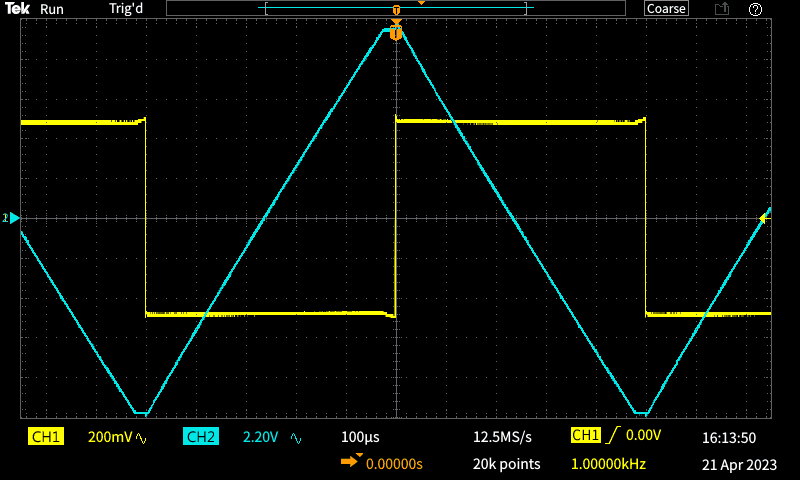
\includegraphics[width=0.75\textwidth]{TEK00000.PNG}
    \caption{Darstellung einer Rechteckspannung und einer integrierten Dreiecksspannung}
    \label{fig:Versuch2/Darstellung einer Rechteckspannung und einer integrierten Dreiecksspannung}
\end{figure}

\newpage
In der Abbildung \ref{fig:Versuch2/Darstellung einer Dreieckspannung und einer integrierten Sinusförmigenspannung} ist der Verlauf der Dreiecksspannung und der intrigierte Verlauf der Dreiecksspannung, welche in diesem Falle Sinus förmig ausfällt, aber keine Sinusfunktion abgebildet. Die Eingangsspannung $U_1$ wird wieder über den Channel 1 dargestellt und das sinusförmige Integral über den Channel 2. Hier kann man auch wieder die Aufmerksamkeit auf den Triggerpunkt richten, wo Sicht bar wird, dass der Hochpunkt des Integrals der Wendepunkt, der Dreieckspannung ist sowie der darauffolgende Tiefpunkt ein weiterer Wendepunkt der Dreiecksspannung befindet.    
\begin{figure}[H]
    \centering
    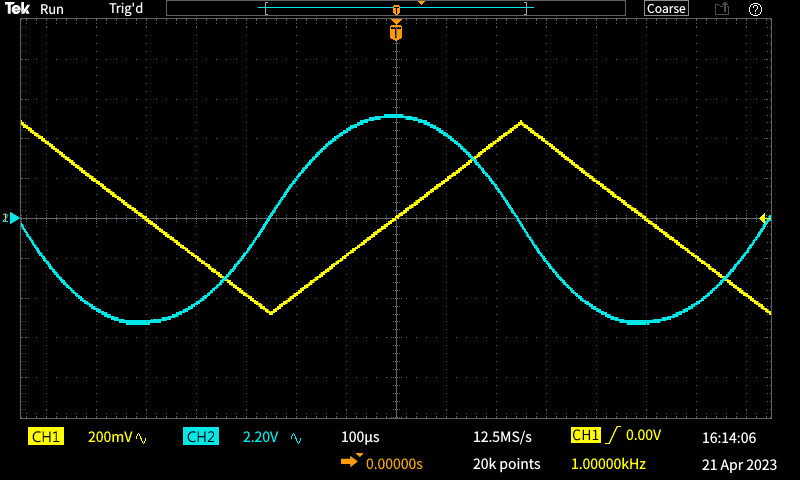
\includegraphics[width=0.75\textwidth]{TEK00001.PNG}
    \caption{Darstellung einer Dreieckspannung und einer integrierten Sinusförmgenspannung}
    \label{fig:Versuch2/Darstellung einer Dreieckspannung und einer integrierten Sinusförmigenspannung}
\end{figure}
In der Abbildung \ref{fig:Versuch2/Darstellung einer Sinusspannung und einer integrierten Cosinusförmigenspannung} ist der Verlauf der Sinusspannung abgebildet und der intrigierte Verlauf der Sinusspannung. Dieser ist auf der Abbildung Cosinus förmig und zeit wie in den anderen Abbildungen durch seine Hoch- und Tiefpunkte die Wendestellen der Sinusspannung.      
\begin{figure}[H]
    \centering
    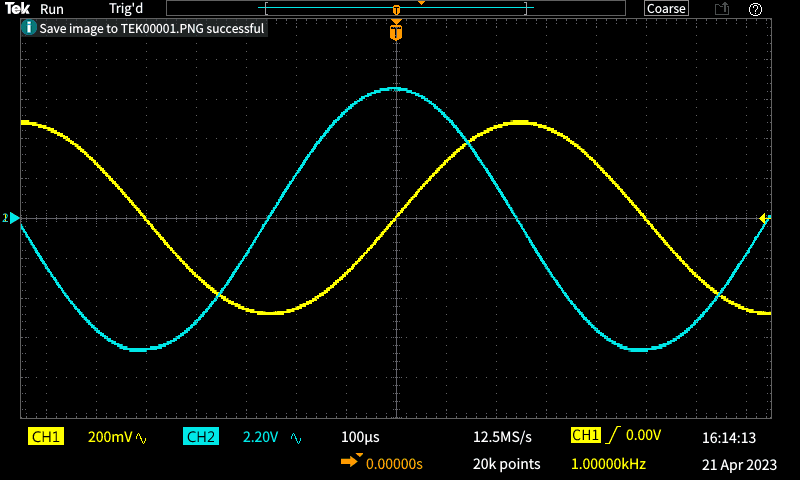
\includegraphics[width=0.75\textwidth]{TEK00002.PNG}
    \caption{Darstellung einer Sinusspannung und einer integrierten Cosinusförmigenspannung}
    \label{fig:Versuch2/Darstellung einer Sinusspannung und einer integrierten Cosinusförmigenspannung}
\end{figure}
\subsection{Frage 2:} Diskutieren Sie die zeitlichen Verläufe von $U_1$ und $U_2$ für die drei Fälle und verglichen Sie diese mit den theoretischen Erwartungen auch im Hinblick auf die Phasenlage.
Der zeitliche Verlauf in der Abbildung\ref{fig:Versuch2/Darstellung einer Rechteckspannung und einer integrierten Dreiecksspannung} zeigt, wie die Spannung in $U_2$ abfällt bis zur Nullstelle von $U_1$ und  von dahin ansteigt bis zur nächsten Nullstelle und dies in einem Wechsel. Dies lässt sich auch bei den Abbildungen \ref{fig:Versuch2/Darstellung einer Dreieckspannung und einer integrierten Sinusförmigenspannung} \ref{fig:Versuch2/Darstellung einer Sinusspannung und einer integrierten Cosinusförmigenspannung} beobachten. Denn bei der Abbildung \ref{fig:Versuch2/Darstellung einer Dreieckspannung und einer integrierten Sinusförmigenspannung} läuft über den Channel 1 Dreiecksspannung, welche intrigiert eine Sinus artige Form annimmt, wo wider die Nullstellen des Integrals die Hoch- und Tiefpunkte die Nullstellen  . Theoretisch ist dies auch zu erwarten, da die $f(x)=0$ die Hoch- und Tiefpunkte der Ableitung zeigt und $f´(x)=0$ zeigt die Hochpunkte von $f(x)$ wodurch sich theoretisch der Verlauf der integrierten Spannung voraussagen lässt, um die Wendepunkte genau zu bestimmen, müsste man jetzt noch $f´(x)$ nochmal intrigieren, um diese zu erhalten. 





